\section{Algorithm}\label{sec:optimization}

\comments{
Assuming every face in the carton model is rigid, which means the interior angle in each plane stays the same.  
%
Furthermore, planes are connected by hinges at the boundary of patches, and the planar layout has its front and back.}

In this section, we explain our algorithm in detail. 
Initially, assume that the 2D layout $\mathcal{L}$ lies on the $XOY$ plane, so that each vertex $\mathbf{v}_i(x_i,y_i,z_i)$ in $V$ has $z_i=0$. 
Each face in $F$ has a normal $\mathbf{n}_i=(0,0,1)^T$.
%
In the first step of our algorithm, our system automatically {\color{blue}{folds the original flat mesh into a rough model by assigning a specific angle to each folding edge.}}
%computes the normal of the desired 3D carton based simple rules of orthogonality and parallelism.
In the second step, the carton shape is refined based on a set of potential geometric constraints.

\subsection{Shape Initialization}\label{sec:initialization}


%\cxj{re-write this section. Describe clearly about the parameters, the objective, and methods. }
%In this section we explain the reason why using a specific angle to each fold edge, and constructing our initialized model. 

A general process for humans to fold a carton starts from folding each edge by a rough angle and then connecting close vertexes to obtain a box-like shape. 
Naturally, we first fold the 2D layout by assigning a rotation angle to each pair of adjacent faces to get a rough shape, instead of directly computing the vertex coordinates.
%The basic idea is to interpret the folded state of a box as a series of rotation angles along each edge, and by setting specific value of angles which is $\pi/2$, we can have a rough model to assist the later optimization.
%	
Observed from existing data in the Internet, most of the traditional cartons are cuboid for holding files or delivering daily supplies. 
Although there is a recent trend to design more complicated layouts to attract consumers, the shape of these unusual cartons is similar to boxes as their functions are still packaging commodity. 
%
Therefore, we choose $\pi/2$ as the initial value of the rotation angle to each folding edge. 
%
First, a face graph of a layout is constructed, as shown in Figure~\ref{fig:midresult} (a).
Each face is a node, and there is an edge between two faces if they are connected by a folding edge.
%
The faces in the 2D layout are recursively folded in a breadth-first manner.
Starting from the face with the maximal area, our system folds all its adjacent faces by rotating them around their connecting edge by $\pi/2$, and then continues to others. 
Figure~\ref{fig:midresult} illustrates the folding process of a cuboid carton. 

\begin{figure}[ht]
	\centering
	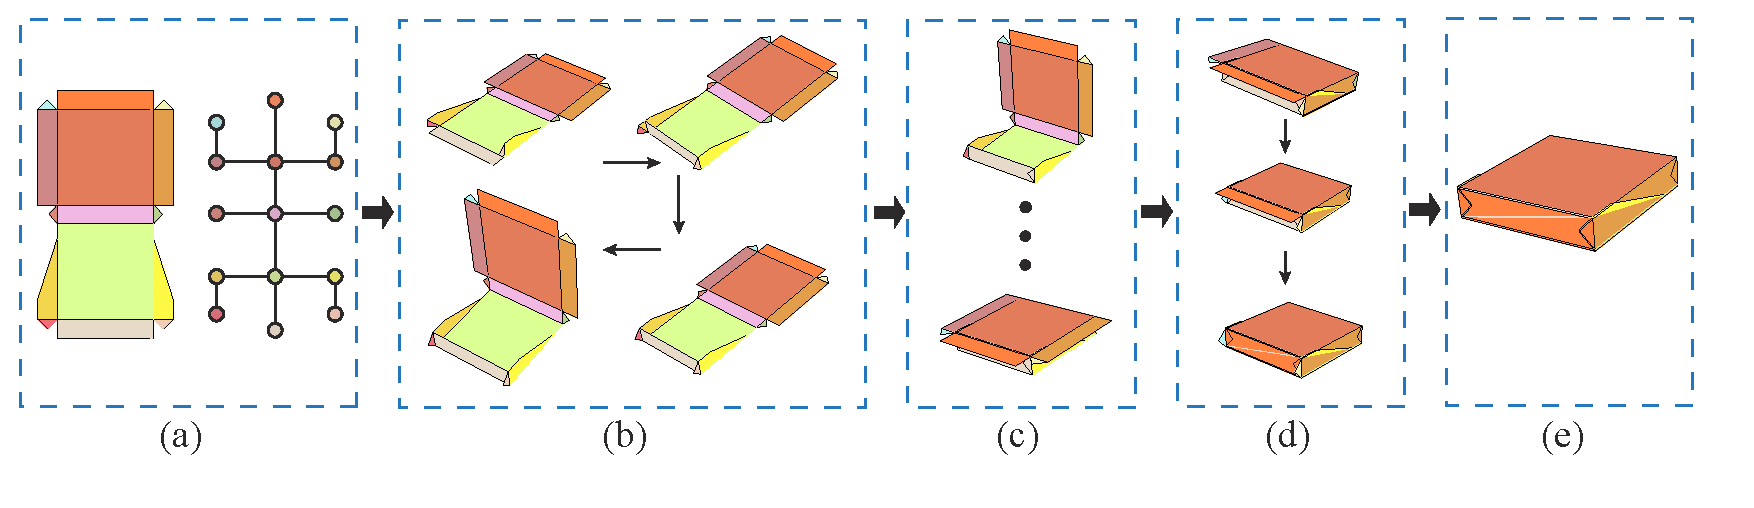
\includegraphics[width=0.9\textwidth]{images/midresult}
	\caption{A rough 3D shape is obtained by folding each face by $\pi/2$ in the 2D layout (a) in a breadth-first manner, starting from the face with the maximal area. (b), (c), (d) and (e) are the different folding stages in the initialization step.}
	\label{fig:midresult}
\end{figure}


{\color{blue}{The following two figures}} shows a group of results generated by simply folding faces by $\pi/2$.
Traditional cartons in cuboid shapes could reach an ideal state, as Figure~\ref{fig:initial-automatic} shows.
However, many complicated designs still need refinement, such as the four examples in Figure~\ref{fig:initial-need-improvement}. 
Take the hexagonal box as an example, the 3D model can be improved by simply snapping the small paste faces to its nearby faces. %
%
As a result, we provide an suggestive interface by automatically detecting potential geometric modifications in the rough carton shape for users to explore.
%interactively allow users to add these constrains into our system and optimize to a desired model, as described in the following section.

\begin{figure}
	\centering
	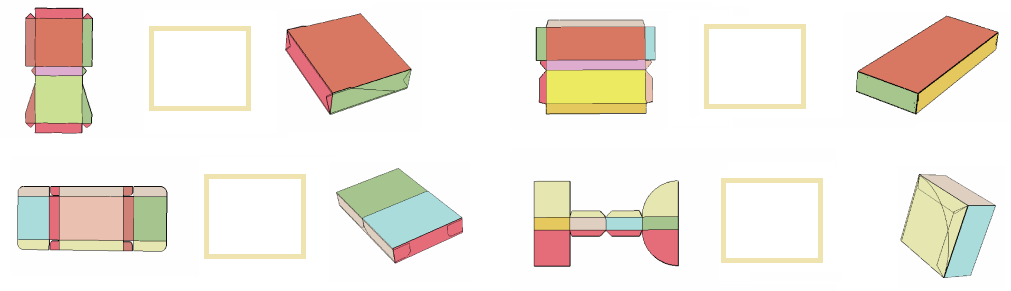
\includegraphics[width=0.9\textwidth]{images/initial-auto.png}
	\caption{Four examples of carton models that can be fully automatically generated from 2D layouts by folding each edge with a fixed angle $\pi/2$. }
	\label{fig:initial-automatic}
\end{figure}


\begin{figure}
	\centering
	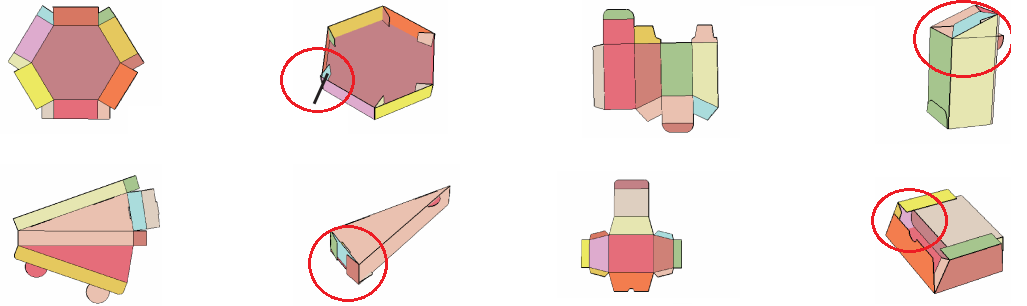
\includegraphics[width=0.9\textwidth]{images/initial-improve.png}
	\caption{Four examples of the carton models that need shape improvement. While the shapes are not cuboid, using a fixed angle $\pi/2$ leads to non-closed shape and loose structure. }
	\label{fig:initial-need-improvement}
\end{figure}
%%%%%%%%%%%%%%%%%%%%%%%%%%%%%%%%%%%%%%%%%%%%%%%%%%%%%%%%%%%%%%%%%%%%%


\subsection{Shape Refinement}\label{sec:refinement}

%there is still a need to refine the results that have not folded into pleasing results. 
Though not perfect, the initial 3D shape provides a good start point for generating the final carton model. 
%
To further refine the 3D shape, the 3D coordinates of all the vertexes are then refined based on a set of shape constraints, such as vertex merging, face pasting, and so on.
%
%the main idea is to prescribe the shape constrains by a set of vertexes of the polymesh. 
%Moreover, with the extra information acquired from user interaction, we can finally construct the desired 3D realization.
In this step, the coordinate of vertexes are chosen as our objective instead of angles on folding edges, mainly because that the geometric constrains in 3D shapes can be more simply and intuitively represented by 3D vertexes.
% and we can implement the algorithm introduced by Bouaziz et al. easily~\cite{Bouaziz:2012:SSD:2346796.2346802}.
 

%\subsection{Aided Detection}

%While the initial 3D model with simple angle folding provides a rough idea about the carton shape, 
A suggestive interface is provided to users for efficiently explore better carton shapes, as described later in Sec.~\ref{sec:interaction}. 
%
Once the user selects a suggested shape refinement operation, we optimize the 3D shape based on a series of geometric constraints.
%We now introduce the constrains used in our construction method:
Given the current mesh whose vertex positions are defined as $\{\vo_i\}^{N}_{i=1}$, a new mesh with the same topology but new vertex positions $\{\vn_i\}^{N}_{i=1}$ is constructed.
%
The geometric constraints can be classified into two groups, \cxj{shape rigidity constraints and shape modification constraints}.
% 
First, to keep the rigidity of each face, the constraints including edge length constraint, coplanarity, and face rigidity, which are corresponding to similarity constraint and plane constraint described in \cite{Bouaziz:2012:SSD:2346796.2346802}. 
%
Second, once two vertexes or two faces are confirmed to be merged to modify the rough shape, more constraints are added. 
%
Each constraint is defined as following.  

\comments{
\paragraph{Edge length constraint.} 
For each edge in $\{e_j\}_{j=1...M}$, its length should be preserved when refine the carton shape.
Hence, its two endpoints $\mathbf{v}_{js}$ and end point $\mathbf{v}_{jt}$ should satisfy 
\begin{equation}
||\mathbf{v}_{js} - \mathbf{v}_{jt}||^2 = ||\mathbf{\hat{v}}_{js} - \mathbf{\hat{v}}_{jt}||^2.
\label{equ:edge}
\end{equation}
%to ensure that the length of each edge stays the same.
}


\paragraph{Face rigidity} 
Each face keeps its shape unchanged during folding. This constraint is defined by keeping the length of each line connecting any pair of points $\mathbf{v}_{a}, \mathbf{v}_{b}$ on the face the same.
\begin{equation}
||\mathbf{v}_{a} - \mathbf{v}_{b}||^2 = ||\hat{\mathbf{v}}_{a} - \hat{\mathbf{v}}_{b}||^2.
\label{equ:plane}
\end{equation}




\paragraph{Coplanarity} {For each face in  $\{f_k\}_{k=1,\dots,P}$, the coplanarity constraint specifies all vertexes in a face should always lie on a plane. 
We can compute the sorted eigenvectors $\mathbf{U} = [\mathbf{e}_1, \mathbf{e}_2, \mathbf{e}_3]$ of the $ 3 \times 3$ covariance matrix $\mathbf{C}^T\mathbf{C}$ where $\mathbf{C} = \{\mathbf{v}_{kj}\}_{j=1}^{N_k}$, $\mathbf{v}_{kj}$ is the $j$th vertex among $N_k$ vertexes in the face. Plane projection can be obtained by removing the last column of $\mathbf{U}$. 


If a set of shape modification operations, such as vertex merging and face pasting, are selected, more constraints are added to optimization vertex positions. 
%
%and one of the interaction is to choose the right given suggestion including points needed to be merged together. As for the point information, the constrains can be written like:

\paragraph{Merging vertexes} 
For any two vertexes $\mathbf{v}_p$ and $\mathbf{v}_q$ that are selected to be merged as the same vertex, we have 
\begin{equation}
\mathbf{v}_p - \mathbf{v}_q = \mathbf{0}.
\label{equ:point}
\end{equation}
%if these two points $\mathbf{v}_p$, $\mathbf{v}_q$ need to be moved into the same place. 

\paragraph{Face pasting} \cxj{check if this is right. }
%If a smaller face $f_a$ is snapped to a larger face $f_b$, for each vertex $\vn_i$ in the face $f_b$, we have
%\begin{equation} \label{eq:face-paste}
%\vn_i \cdot \mathbf{n}_a = 0,
%\end{equation}
%where $\mathbf{n}_a$ is the normal of the face $f_a$.
{\color{blue}{If two faces $f_a$ and $f_b$ need to snap together, the whole vertexes of these two faces should satisfy coplanarity constrain.}}


When the above constrains still lead to an ill-posed problem, soft constraints will be added to keep the original positions of the vertexes that are not relative to the shape modification. 

\paragraph{Irrelevant vertexes} For the vertexes $\{\mathbf{v}_i\}$ are not in the same plane with any vertex for merging or face pasting, they should stay at their original location. 
We add these soft constraints by adding a small weight $w$, which is set 0.001 in our experiments to the following equation. 
\begin{equation}
\mathbf{v}_i - \mathbf{\hat{v}}_i = 0.
\label{equ:irrelevant}
\end{equation}

Combining the above constraints, the new vertex locations can be solved using the \cxj{XX method, cite the paper.}
%
Figure~\ref{fig:shaperefinement} shows two examples of shape refinement by merging three vertexes and pasting two faces respectively. 

\comments{
\cxj{My suggestion on Figure 4: (a)(b) 3D shape before/after vertex merging, highlight the vertexes. (c)(d) 3D shape before/after face pasting.}

Figure~\ref{fig:constrain} illustrates the necessity of basic three constrains.
\cxj{More detailed explaination on the figure. Explain the three constraints in the figure.}
{\color{blue}{When we merge three vertexes circled in red Figure~\ref{fig:constrain} (b) into one location, the optimized model is generated under basic constraints shown in Figure~\ref{fig:constrain}}. The model shown in Figure~\ref{fig:constrain} (d) (e) and (f) are the results after optimizing without edge length constrain, coplanarity and face rigidity constrain separately. Without edge length constrain, the two red edges have been stretched Figure~\ref{fig:constrain} (d), the face surrounded by red lines Figure~\ref{fig:constrain} (e) is not a standard plane without coplanarity, and the face surrounded by red lines in Figure~\ref{fig:constrain} (f) has been deformed without face rigidity.}

\begin{figure}
	\centering
	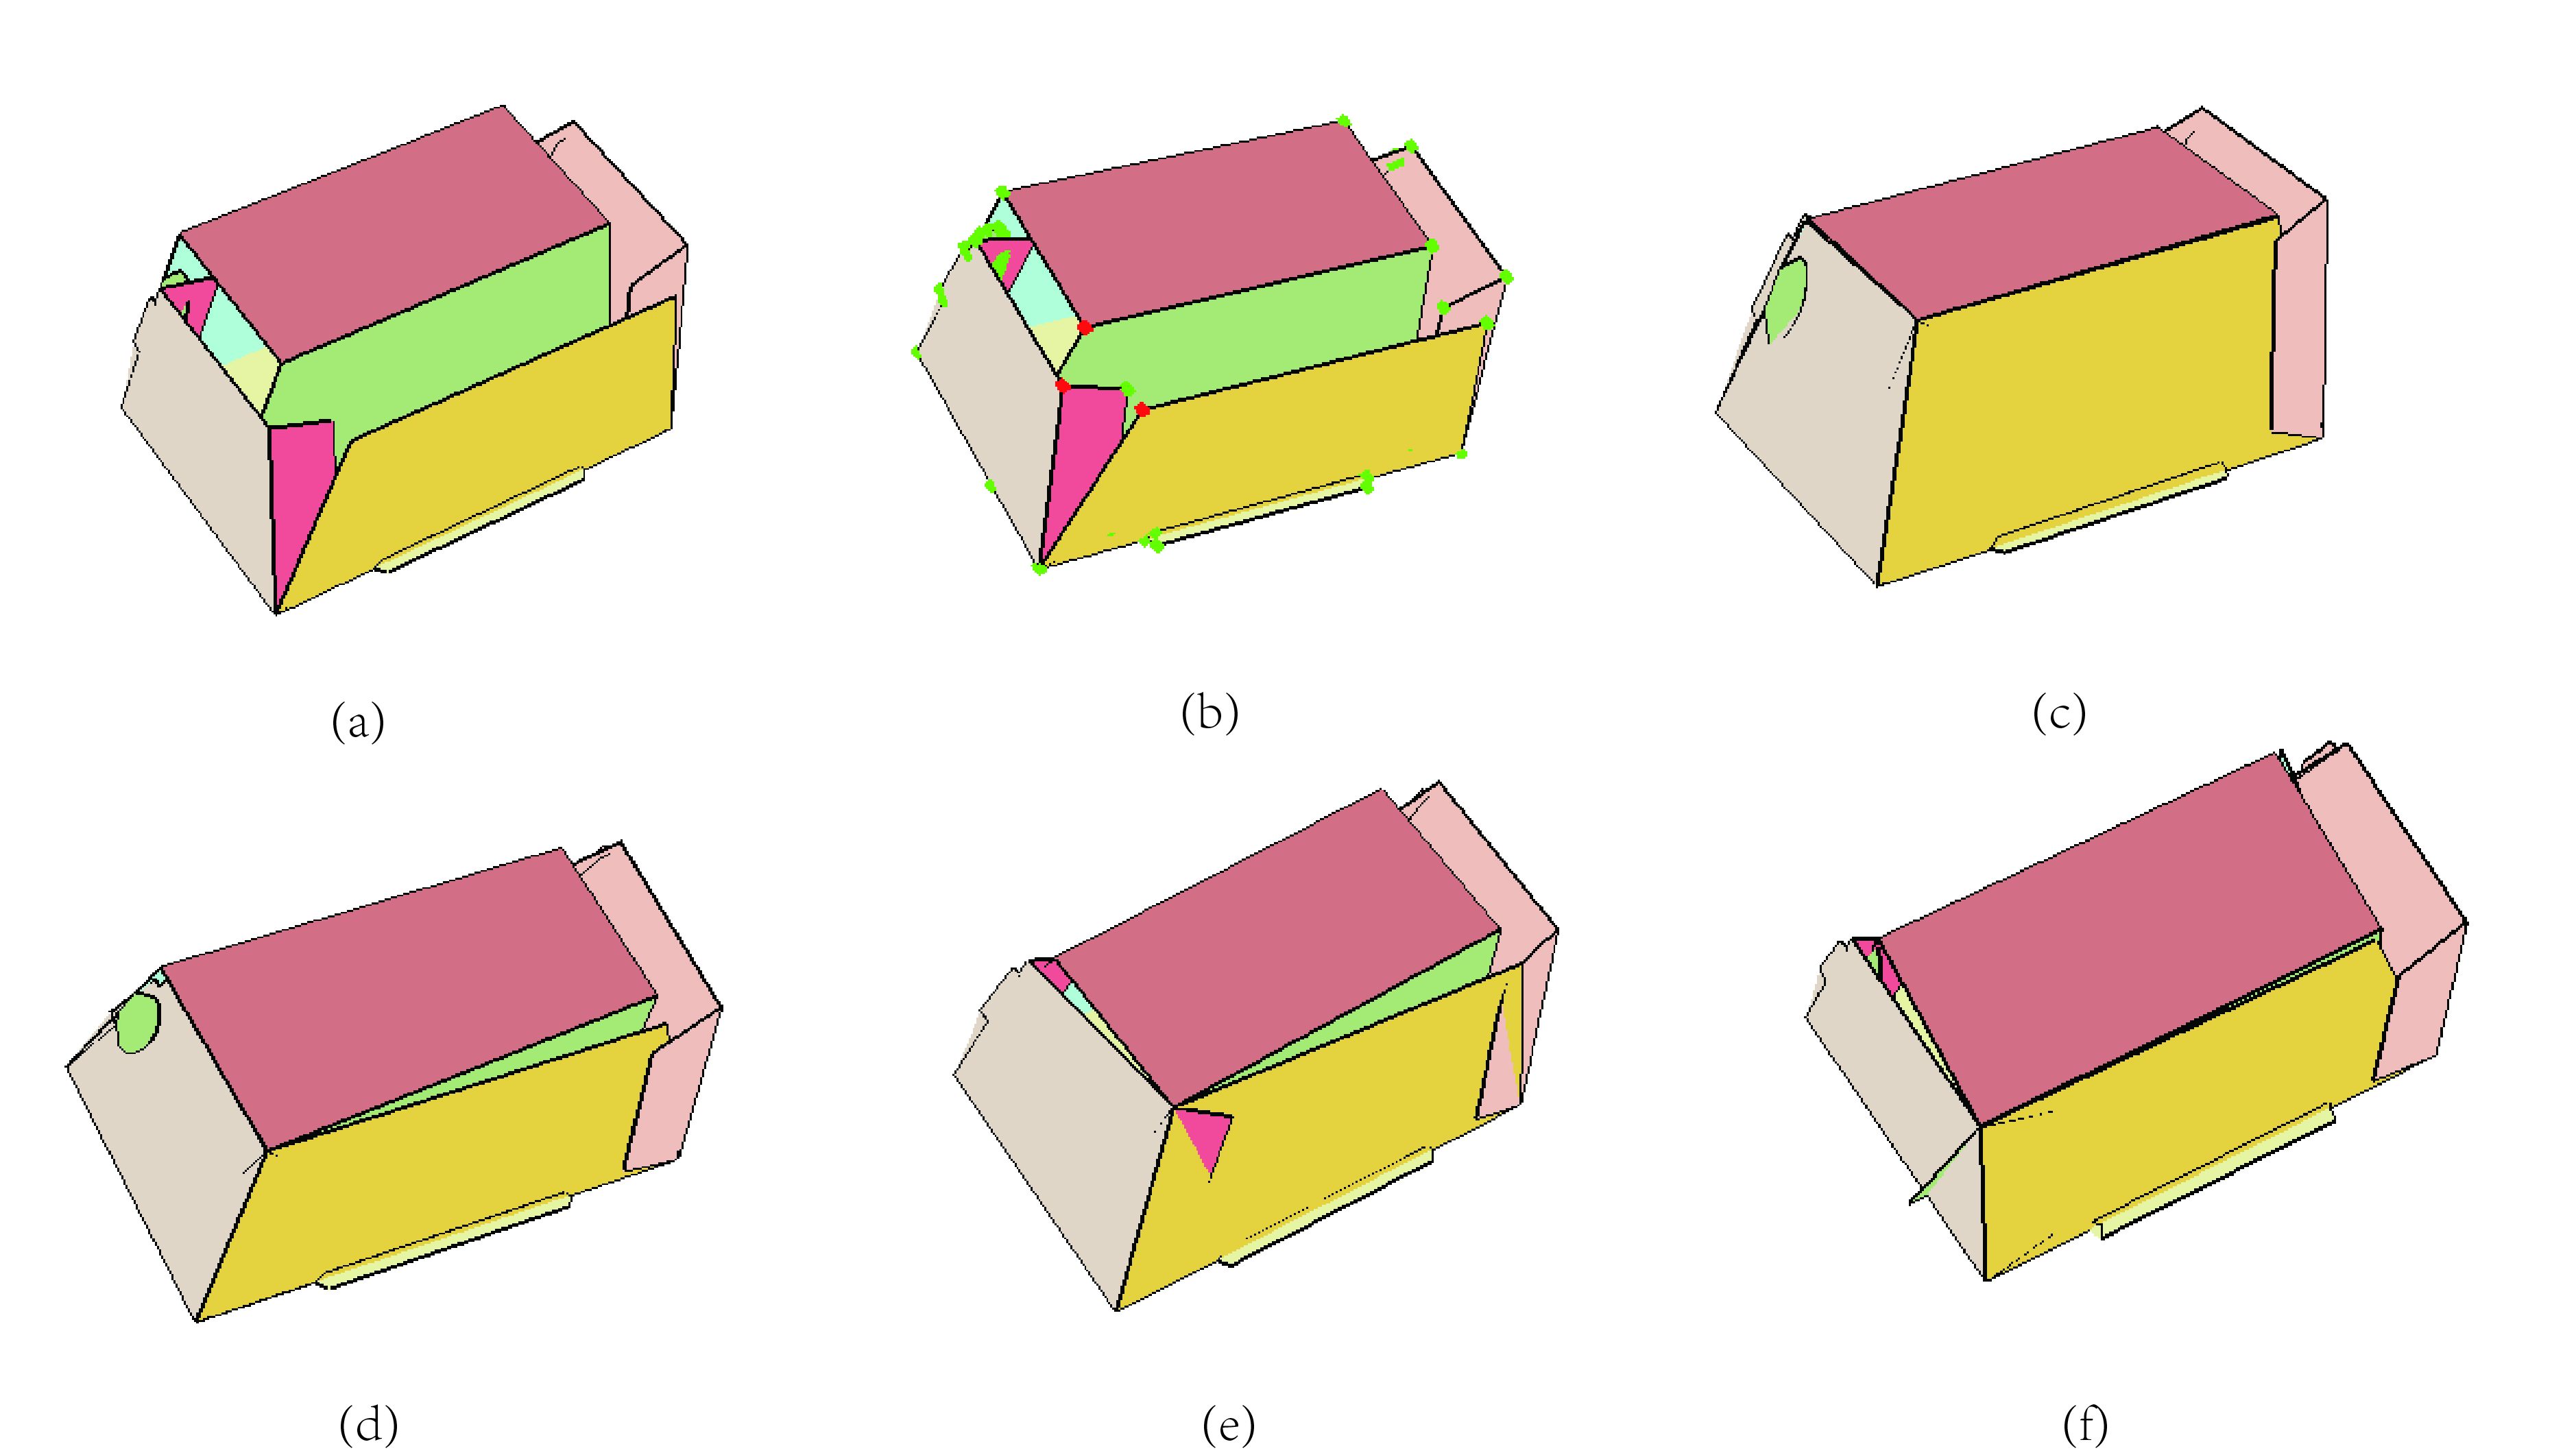
\includegraphics[width=0.9\textwidth]{images/constrain.jpg}
	\caption{Given an initial shape~(a), by merging the three vertexes marked in red~(b), basic three shape constrains can lead to the optimization result~(c). The bottom three are the results optimized lack of edge length constraint, coplanarity and face rigidity separately, compared to~(c), the results can not keep the basic shape well. Without edge length constrain, the two red edges have been stretched (d), the face surrounded by red lines (e) is not a standard plane without coplanarity, and the face surrounded by red lines in (f) has been deformed without face rigidity.}
	\label{fig:constrain}
\end{figure}
}


\begin{figure}
	\centering
	\subfigure[Vertex Merging]{
		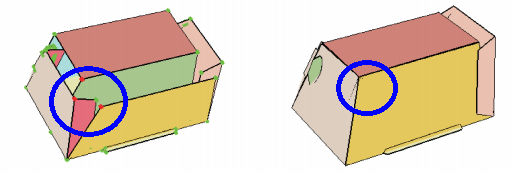
\includegraphics[width=0.45\columnwidth]{images/vertexMergingBA.png}
		\label{fig:vertexmergingBeforeAfter}
	}
	\subfigure[Face Pasting]{
		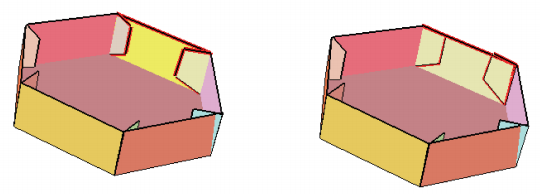
\includegraphics[width=0.45\columnwidth]{images/faceMergingBA.png}
		\label{fig:facemergingBeforeAfter}
	}
	\caption{3D shape refinement based on merging vertexes (a), or pasting faces (b). The locations where the 3D shape changes are highlighted in blue.  }
	\label{fig:shaperefinement}
\end{figure}
